\documentclass[titlepage]{article}
\usepackage{graphicx}
\usepackage{tikz}
\usepackage{lipsum}
\usepackage{lmodern}
\usepackage[T1]{fontenc}
\usepackage[utf8]{inputenc}
\usepackage[french]{babel}
\usepackage[left=2.5cm, right=2.5cm, top=2cm, bottom=2cm]{geometry}
\usepackage{graphicx}
\usepackage[colorlinks, citecolor=blue, urlcolor=blue, linkcolor=blue, linktocpage=true]{hyperref}
\usepackage{amssymb, amsmath, amsfonts, amsthm}
\usepackage{float}
\usepackage{xcolor}  

\begin{document}

\begin{titlepage}

    \begin{tikzpicture}[remember picture,overlay]
    
       \node[inner sep=0pt] at (current page.center) {
\includegraphics[width=\paperwidth,height=\paperheight]{fond.png}};
        
        \begin{scope}[shift={(current page.center)}]
        
            \node[align=center, text width=10cm, black] at (7, 2) {  
                \Large\textbf{Fait le 12 novembre 2023}};
            \node[align=left, text width=10cm, black] at (-5, -4.3) {
                \Large\textbf{Rapport d'étude}\\
                \vspace{0.5cm}
                \Large\textbf{SAE 3-03 : Description et prévision de données temporelles}\\
                \vspace{6cm}};
            \node[align=left, text width=10cm, black] at (-5,-5) {
                \Large\textit{R3 - 14 : Séries chronologiques}\\
                \vspace{2cm}};
            \node[align=right, text width=10cm, black] at (5,-4.5) {
                \Large\textit{Auteurs du rapport :}\\
                \vspace{1cm}};
            \node[align=right, text width=10cm, black] at (5,-7.7) {
                \Large\textbf{Valentin Rieu\\Amadou Moussa Sow\\Clément Husson\\Théo Brugel\\}
                \vspace{1cm}};
                 \vspace{2cm};
             \node[align=right, text width=10cm, black] at (5,-11) {
                \Large\textit{Enseignant référent :\\}
                \vspace{1cm}};
            \node[align=right, text width=10cm, black] at (5,-12.5) {
                \Large\textbf{Paul-Marie Grollemund}
                \vspace{2cm}};
                
        \end{scope}
        
    \end{tikzpicture}
    
\end{titlepage}

\newpage
\null
\newpage

\tableofcontents

\newpage
\null
\newpage

\section*{Introduction}
\addcontentsline{toc}{section}{Introduction}
\vspace{0.5cm}

Dans le cadre de notre projet de série chronologique, nous devons mener une étude statistique sur l'analyse de la circulation automobile entre une ville et une route nationale qui l'entrave.
\\
Pour ce faire, un fichier csv intitulé, "routeintersection.csv", répertoriant toutes les données automobiles du 1er novembre 2015 au 30 juin 2017 nous a été fourni. 
\\
L'objectif est donc d'apporter des réponses aux problématiques posées à  partir de nos compétences statistiques et informatiques qui seront directement mises en application sur le logiciel RStudio.
\vspace{0.5cm}
\\
La configuration entre cette ville et la route est marquée par trois intersections provenant directement de la ville ($I_1, I_2, I_3$), de trois entrées ($E_1, E_2, E_3$) et trois sorties depuis la nationale ($S_1, S_2, S_3$). Pour pallier d'éventuelles situations de désengorgement des entrées, une quatrième intersection a été construite le 1er janvier 2017 par la municipalité. 
\\
Pour déterminer l'importance de cette dernière intersection, nous devons obtenir des éléments de réponses concrets. Pour ce faire, nous utiliserons la base de données fournie pour nous servir de ces nombreuses données. 
Il contient une première colonne intitulée "Date", qui  enregistre le jour et l'heure de passage de chaque véhicule sur une intersection. 
De plus, nous avons une deuxième colonne "Intersection", dans laquelle les quatre intersections sont répertoriées. 
Enfin, il y a une colonne nommée "vehicule" qui comptabilise le nombre de véhicules qui sont passés par une intersection à  un instant T.
\\
\vspace{0.5cm}
\\
L'objectif de cette étude est de répondre à trois problématiques qui sont les suivantes : 

\begin{itemize}
    \item Evaluer s'il y a eu un désengorgement des trois premières intersections, suite à la mise en place de la quatrième intersection I4;
    \item Indiquer s'il y a eu une circulation anormale avant ou après le 1er janvier 2017 et indiquer s'il semble y en avoir plus avant ou après;
    \item Faire une prévision du nombre de véhicules passant par chacune des quatre intersections pour la journée suivante. Il faudra faire la même chose pour le mois suivant.
\end{itemize}
\vspace{0.5cm}

Pour ce faire, nous allons devoir procéder à  un traitement efficace des données et tenter de "remodéliser" le jeu de données de sorte à  pouvoir travailler avec les éléments qui nous intéressent. Ces données permettront notamment de distinguer une cassure et mettre en avant, tant graphiquement qu'au travers de calculs, des différences avec l'ajout de la quatrième intersection. 
\vspace{0.5cm}
\\
Nous vous laissons donc prendre connaissance des différents calculs qui ont été réalisés et les interprétations qui en ont découlé.

\newpage

\section{Prétraitement}

Le fichier csv que nous avons est organisé de la manière suivante. Chaque ligne contient
le nombre de véhicules en fonction d'une heure et d'une
intersection. Donc les différentes intersections sont
mélangées et une ligne ne correspond pas à une heure
précise, le tableau de la figure~\ref{figure:fig1} nous donne un échantillon fictif du fichier.
\vspace{0.5cm}

\begin{figure}[H]
\centering

\begin{tabular}{|c|c|c|}
\hline
Date & Intersection & Nombre\\
\hline
2015-11-03 $00 {:} 00 {:} 00$ & $I_1$ & 12\\
2015-11-03 $00 {:} 00 {:}  00$ & $I_2$ & 15\\
\vdots & \vdots & \vdots\\
2015-11-03 $01 {:} 00 {:}  00$ & $I_1$ & 15\\
2015-11-03 $01 {:} 00 {:}  00$ & $I_2$ & 23\\
\vdots & \vdots & \vdots\\
\hline
\end{tabular}

\caption{Echantillon fictif du tableau de données}
\label{figure:fig1}
\end{figure}

\vspace{0.5cm}
Nous avons décidé de garder ce tableau pour
tracer les graphiques et d'en créer un autre pour faire
des calculs. Ce dernier est une liste qui contient un 
tableau pour chaque intersection. Deplus, nous avons
remarqué que la colonne qui comptait le nombre de
véhicules contenait des nombres décimaux, nous avons
décidé d'arrondir les valeurs avec leur partie entière
par excès. Grâce à un arrondi effectué avec la partie entière par excès,
toutes les valeurs sont arrondies à l'entier supérieur et non pas en fonction
du cas, ce qui permet d'harmoniser les valeurs.\\

Pour lisser la série, nous avons effectué un lissage par moyenne mobile
avec $k = 12$. Nous avons choisi un lissage par moyenne mobile car
un lissage exponentiel peut ne pas être précis en cas de fortes
variations, ce qui est le cas ici. Nous nous sommes permis de prendre
le paramètre $k$ égal à 12 car il y a beaucoup de valeurs et donc
l'effet de bord ne nous dérange pas trop.

\newpage
\section{Analyses}
\subsection{Désengorgement des intersections}

La figure~\ref{figure:fig2} représente la tendance linéaire du nombre de véhicules passant par chaque intersection.

\begin{figure}[H]
\centering
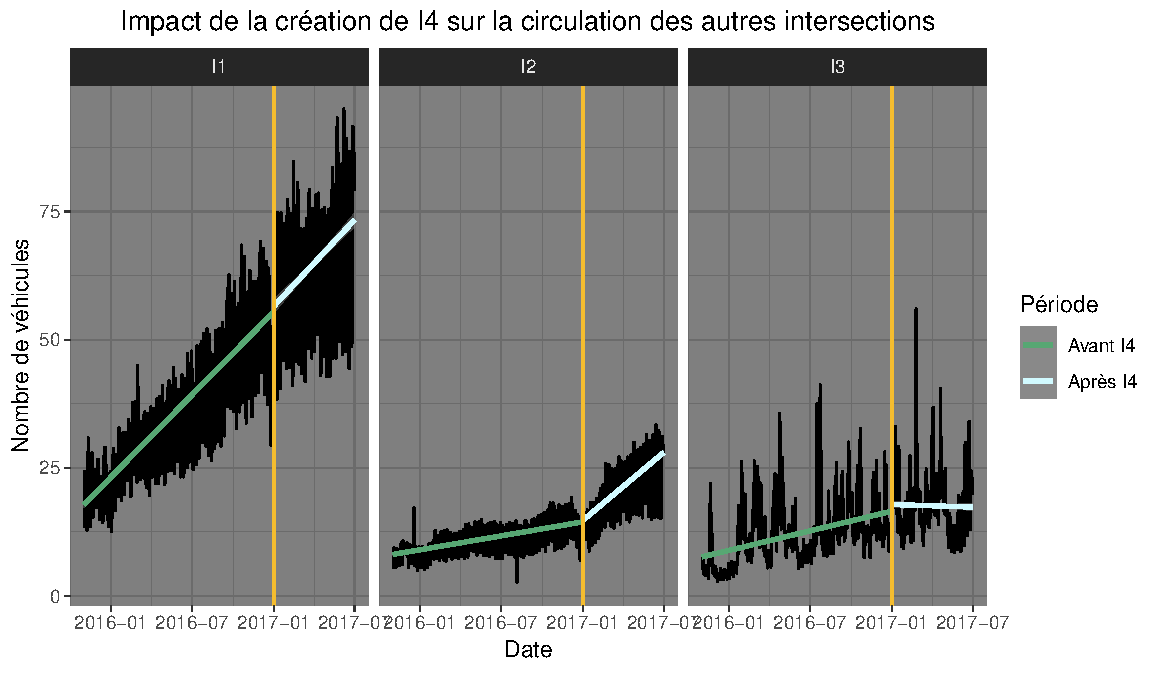
\includegraphics[scale=0.55]{vehicule_I4.pdf}
\caption{Tendance linéaire du nombre de véhicules passant par chaque intersection avant et après la mise en place de $I_4$}
\label{figure:fig2}
\end{figure}

Visuellement, nous pouvons déjà remarquer que les trois séries lissées ont une tendance linéaire à la hausse,
et la troisième semble plus chaotique. Pour la deuxième, après la mise en place de $I_4$, la tendance
semble partir encore plus à la hausse, et pour la première nous ne voyons pas de changements importants.
Les 6 équations de régressions sont : $y_{1, 1} = 0.003668019t + 17.826934818, y_{1, 2} = 0.002853456t + 27.413253948,
 y_{2, 1} =  0.0006179654t + 8.0832705352, y_{2, 2} = 0.00227276t - 8.53153529,
y_{3, 1} = 0.0008698147t + 7.5982644087, y_{3, 2} = -0.000122173t + 19.142058253$.
Donc pour $I_1$, il ne semble pas y avoir de différences importantes, mais pour $I_2$, nous voyons bien une augmentation du
coefficient directeur et pour $I_3$, la tendance s'inverse. Pour vérifier qu'il y a bien une cassure à cette date, nous avons
réalisé trois tests de Chow. Les $p$-valeurs que nous obtenons sont respectivement $p_1 = 9.76 \cdot 10^{-3},
p_2 = 0$ et $p_3 = 9.50 \cdot 10^{-15}$. Si nous choisissons un risque $\alpha = 5$ \%, les trois $p$-valeurs sont
largement inférieures au risque, on en conclut avec un risque de 5 \% que la date de mise en place de $I_4$ est une cassure pour
les trois séries. Cependant, seul $I_3$ semble avoir été légérement désengorgé.

\begin{figure}[H]
\centering
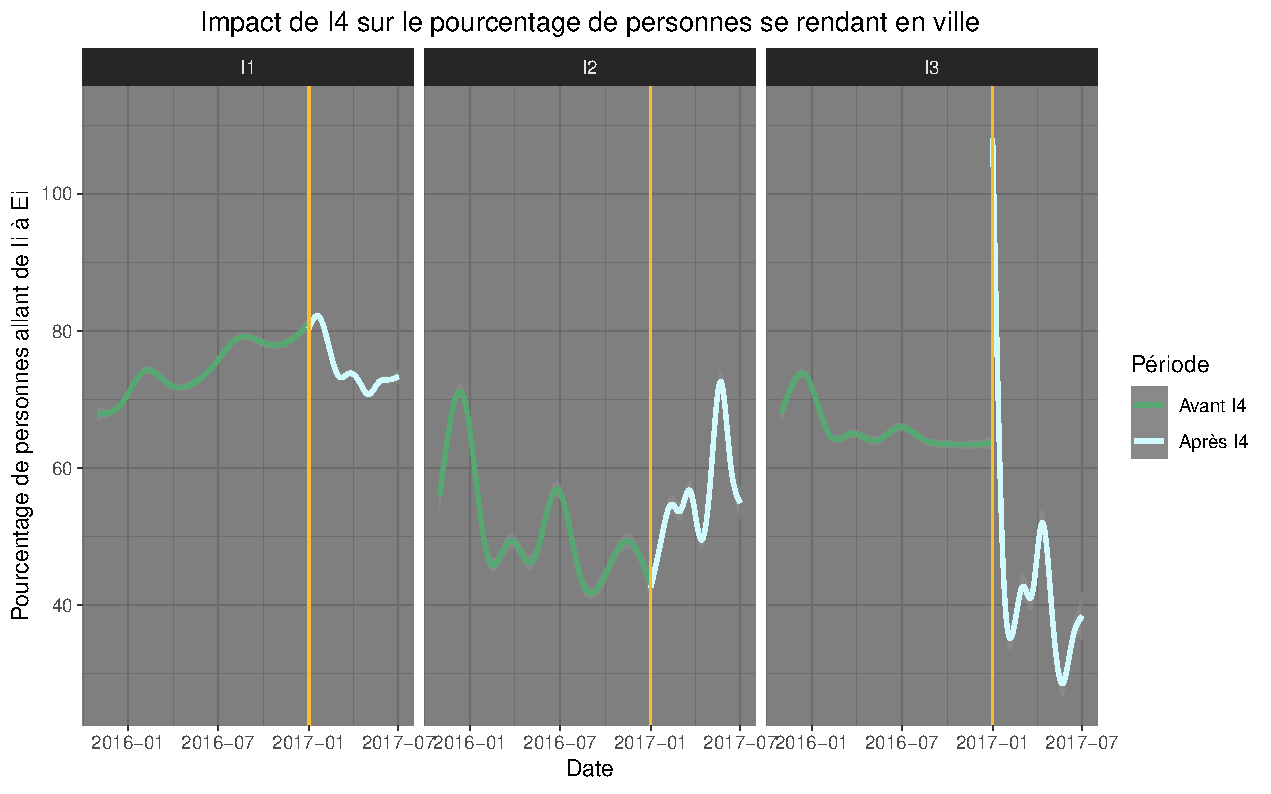
\includegraphics[scale=0.48]{pourcentage_intersection.pdf}
\caption{Lissage avec la méthode GAM de l'évolution du pourcentage de 
personnes qui se rendent de $I_i$ à $E_i$}
\label{figure:fig3}
\end{figure}

Sur la figure~\ref{figure:fig3}, la méthode de lissage utilisée est la \href{https://rdrr.io/cran/mgcv/man/gam.html}{méthode GAM}, car c'est
celle par défaut de la bibliothéque ggplot2 quand il y a beaucoup de valeurs. Pour $I_1$, on observe une légère augmentation pendant quelques
jours, puis la tendance repart à la baisse. Pour $I_2$, on observe une augmentation globale et pour $I_3$, il y a un fort pic puis une descente
globale.

\subsection{Circulation anormale}

Pour détecter où sont les anomalies, ils nous faut d'abord un modèle. Comme nous l'avons vu sur la figure~\ref{figure:fig2}, la première
série lissée semble avoir une tendance linéaire et une période, mais l'amplitude des périodes semble devenir de plus en plus importante, donc
un modèle multiplicatif est adapté. Pour la deuxième, on observe aussi une augmentation de l'amplitude des périodes mais la tendance n'est
pas linéaire, enfin, la troisième série semble très chaotique, et n'a pas de tendance linéaire. Donc pour les trois séries, nous avons ajusté un
modèle mutltiplicatif avec une période de 24, car l'unité de temps est l'heure. Nos 3 modèles semblent bien modéliser l'évolution des séries
car les résidus sont imprédictibles et donc non-modélisables. Nous obtenons des MSE raisonnables : $\text{MSE}_1 = 19.9,\text{ MSE}_2 = 5.3, \text{MSE}_3 = 34.3$,
le $MSE_3$ est plus élevé car nous avons vu que la troisième série semble plus chaotique et donc plus difficile à modéliser.\\

Pour détecter des anomalies, nous avons choisis la méthode des quantiles avec des quantiles à 5 \% et 95 \%. En faisaint un rapport entre le
nombre d'anomalies sur une période et une intersection données et le nombre d'anomalies total pour une l'intersection en question, nous obtenons
la part que représente les anomalies à une période. Donc pour $I_1$ et $I_2$ il y a plus d'anomalies après la mise en place de $I_4$ avec 53 \% des
anomalies après pour $I_1$ et 58 \% pour $I_2$. Seul $I_3$ a plus d'anomalies avant avec 61 \% des anomalies.

\subsection{Prévisions}

Avec nos modèles, nous avons fait des prévisions pour le jour suivant et pour le mois suivant pour nos 4 intersections. Pour les prévisions par mois,
nous sommes parti du principe que c'est un mois de 30 jours, donc il possède 720 heures. Pour faire des prévisions, nous faisons la somme des prévisions
pour les 24 prochaines heures et pour un mois, la somme des prévisions pour les 720 prochaines heures. Les calculs sont ensuite arrondis car ces valeurs
sont des nombres de véhicules, elles doivent être des entiers. Pour le modèle 1, le jour suivant il devrait y avoir 351 véhicules, et 15711 le mois suivant.
Pour le modèle 2, il devrait y avoit 141 véhicules le jour suivant et 6179 le mois suivant. Pour l'intersection 3, il devrait y avoir 151 véhicules le jour suivant
et 5383 le mois suivant. Et enfin, pour l'intersection 4, il devrait y avoir 36 véhicules le jour suivant et 5137 le mois suivant.

\newpage
\section*{Conclusion et interprétations}
\addcontentsline{toc}{section}{Conclusion}

La mise en place de la nouvelle intersection n'a pas permis de désengorger véritablement les intersections sauf la 3$^{\text{e}}$. Cependant, la 3$^{\text{e}}$
intersection est beaucoup plus chaotique que les autres et par conséquent beaucoup plus compliquée à modéliser. L'effet de la mise en place de $I_4$ sur cette
intersection est minime, il faudrait peut-être attendre plus longtemps pour voir si la tendance à la baisse continue. Par rapport à $I_1$, la mise en place a eu
très peu d'effet, la tendance à la hausse continue. La mise en place de $I_4$ a eu le contraire de l'effet voulu puisque la tendance à la hausse a été
nettement augmenté. Nous pouvons expliquer la baisse sur $I_3$ par les gens qui habitent en ville, ceux qui souhaitaient se rendre à l'Est peuvent le faire
directement sans passer sur $I_3$ mais $I_4$ directement. S'il n'y a pas eu de changement sur $I_1$, cela peut être expliqué par son éloignement par
rapport à $I_4$. Enfin, la hausse sur $I_2$ est peut-être dû à la hausse du nombre de personnes qui rentrent en ville par $I_2$. Nous pouvons aussi
remarquer que la mise en place de $I_4$ a provoqué un effet de nouveauté, ce qui fait baisser la circulation sur les 3 premières intersections les premiers
jours.\\

Pour le pourcetage de personnes qui se rendent en ville, nous observons une légère augmentation pour la première intersection et une augmenation continue
pour la deuxième. $I_3$ a en revanche une très grosse augmentation, sûrement dûe à l'effet de nouveauté. Peut-être qu'une grande partie des personnes
se sont senties désorientées en arrivant sur $I_3$ et ont décidé d'aller en ville, puis elles ont suivis les panneaux pour retrouver la nationale en passant par
$I_4$. Certaines personnes ont peut-être sont peut-être allé jusqu'à $I_3$ pour voir comment était la route maintenant et sont ensuite retourné en ville par
$I_3$ au lieu de leur intersection habituelle. C'est peut-être aussi cela qui a fait augmenter le traffic sur $I_2$, donc tant que les gens qui ne viennent pas
tous les jours en ville ne seront pas passés, il y aurait potentiellement une augmentation.\\

Enfin, la mise en place de $I_4$ a potentiellement modifié le comportement des conducteurs, puisque pour $I_1$ et $I_2$, la plupart des anomalies se
trouvent après la mise en place de $I_4$. L'effet contraire s'est produit pour $I_3$, $I_4$ aurait permis diminuer les différences entre les heures.

\end{document}